\documentclass[a4paper]{article}

\usepackage[english]{babel}
\usepackage[utf8]{inputenc}
\usepackage{amsmath}
\usepackage{graphicx}
\usepackage{epstopdf}
\usepackage{psfrag} 

\usepackage{listings}
\lstset{
  basicstyle=\ttfamily,
  columns=fullflexible,
  frame=single,
  breaklines=true,
}

\title{Udacity Data Analyst Nanodegree Project 1: Explore Weather Trends }

\author{Oliver Kr\"{o}ning}

\date{\today}

\begin{document}
\maketitle

\begin{abstract}
In this project, global temperature data of the recent $\approx 260$ years are analyzed to evaluate global weather trends. Furthermore, the yearly average temperatures of Hamburg, Germany, are examined and local weather trends are derived. Using suitable tools, e.g. Python and SQL, to extract, analyze and interpret the temperature data, a comparison of the local weather development and the global climate change is performed. It is shown, that both, the local and global average temperature, have increased dramatically in the recent years. Thereby, both weather trends exhibit great similarites regarding size and development.  
\end{abstract}

\section{Introduction}
\label{sec:introduction}

Global warming, which is also referred to as global climate change, has been one of the major issues around the world today. The increase of the global temperature creates a number of universal and specific problems according to the environment, e.g. extreme weather events, as well as social systems. Human populations in less developed areas are primarly affected because of negative effects on agriculture and settlements on islands threatened by the rise of sea level. In the recent years, political negotiations and agreements have tried to face the negative global weather trends. Thereby, the specifications and characteristics of global warming can differ by region.
  
\section{Tools}
\label{sec:tool}
To compare the change of temperatures in different regions with global weather developments, a database, which contains local and global temperature data, was given by Udacity. The database provides climate data for nearly every big city around the world. The evaluation in this paper focusses on the local characteristics of weather changes in Hamburg, Germany. With a few exceptions, Hamburg's yearly average temperature is given by the database from 1743 to 2013. Global weather data are presented from 1750 to 2015.
\subsection{SQL}
The Structured Query Language (SQL) is a common and frequently used database language for defining data structures, extracting, editing and deleting data as well as querying database content.

\subsection{Python}
Python is a high-level programming language for general-purpose programming. It provides a good code readability and simplicity due to reduced code syntax and limitation of key words. Python supports both, object oriented and structured programming. Data types are maintained dynamically.\\
In this project, Python's Integrated Development and Learning Environment (IDLE) is used to create, interpret and debug source code in Python 2.6. 

\section{Methods}
\subsection{Data Extraction}
The given databases are processed using SQL within a SQL interpreting workspace on \emph{https://classroom.udacity.com}. Therefore, the global and local temperature data needed for analyzing weather trends are extracted. The global yearly average temperature values are stored in the database \emph{global\_data}. To evaluate and visualize these values and to import them into Python, the data are selected using the commands of Listing \ref{lst:ExtractGlobalData} and saved as the comma-separated values (CSV) file \emph{global\_avg\_temp.csv}.
\begin{lstlisting}[caption={Extract global data from database using SQL},label=lst:ExtractGlobalData]
SELECT * 
FROM global_data
ORDER BY year;
\end{lstlisting}
Analogous to global data, the local average temperature of Hamburg, Germany is extracted from the database \emph{city\_data} as shown in source code in Listing \ref{lst:ExtractLocalData}. Since this database contains data of a number of locations, the selection has to be filtered using a WHERE \dots LIKE command. Finally, the results are saved as \emph{hamburg\_avg\_temp.csv}.
\begin{lstlisting}[caption={Extract local data of Hamburg from database using SQL},label=lst:ExtractLocalData]
SELECT year, avg_temp 
FROM city_data
WHERE city LIKE 'Hamburg'
ORDER BY year;
\end{lstlisting}

\subsection{Data Preparation}
For further data processing, the created CSV files are imported into Python using numpy. Additionally, the data is prepared, to obtain a uniform basis for the comparison between the global and local average temperatures. The procedure and the source code is shown in Listing \ref{lst:DataTreatment}. The CSV files are read out by using numpys \emph{loadtxt()} command.\\
Since the global and local temperature values do not cover the same period of time, the arrays \emph{glob\_temp} and \emph{loc\_temp} have to be cutted and adjusted according to the available values. Thus, yearly average temperature values are provided for each case between a consistent period of time from 1750 to 2013.
\begin{lstlisting}[language=python,caption={Preparation of the imported data within Python},label=lst:DataTreatment]
from decimal import Decimal
import numpy as np
import matplotlib.pyplot as plt
glob_data = np.loadtxt(open("global_avg_temp.csv", "rb"),delimiter=",",skiprows=1)
glob_year = glob_data[:,0]
glob_temp = glob_data[:,1]
glob_min_year = min(glob_year)
glob_max_year = max(glob_year)
loc_data = np.loadtxt(open("hamburg_avg_temp.csv", "rb"),delimiter=",",skiprows=1)
loc_year = loc_data[:,0]
loc_temp = loc_data[:,1]
loc_min_year = min(loc_year)
loc_max_year = max(loc_year)
min_year = max([glob_min_year,loc_min_year])
max_year = min([glob_max_year,loc_max_year])
year = np.arange(min_year,max_year,1)
glob_temp = glob_temp[np.where(glob_year==min_year)[0]:np.where(glob_year==max_year)[0]]
loc_temp = loc_temp[np.where(loc_year==min_year)[0]:np.where(loc_year==max_year)[0]]
\end{lstlisting}

\subsection{Moving Averages}
A rolling average, running mean or moving average describes a simple method for smoothing data or signals within the field of statistics and data processing. Thus, it can be described as a low-pass filter, since high-frequency components are filterd out. For a given window size of $N$, the filter response can be obtained by calculating the mean of the $N$ previous values for each array element. Applying an original time-dependent data vector $x(t)$, the moving average $m_{MA}$ can be written as
\begin{equation}
m_{MA}=\frac{1}{N}\sum^{N-1}_{i=0} x(t-i).
\end{equation}
However, this method suffers from a time lag. Another approach is to apply a centered moving average. In this case, the result for the i-th position is calculated by the mean of the values from $i-(N-1)/2 \dots i+(N-1)/2$.\\
In Python, a function is created to perform the centered moving average as depicted in Listing \ref{lst:MovingAverage}. For further filtering and analyzing procedures, a window size of $N=7$ years is used.
\begin{lstlisting}[language=python,caption={Defining and Applying a function for the centered moving average},label=lst:MovingAverage]
def mov_avg(data,N):
    ma_val = np.array([])
    for i in range((N+1)/2-1,data.size-(N-1)/2,1):
        window = data[i-(N-1)/2:i+(N-1)/2]
        avgval = np.mean(window)
        ma_val = np.append(ma_val,avgval)
    return ma_val
N = 7
glob_temp_ma = mov_avg(glob_temp,N)
loc_temp_ma = mov_avg(loc_temp,N)
year_ma = year[(N+1)/2-1:year.size-(N-1)/2]
\end{lstlisting}

\subsection{Linear Regression}
Additionally to the moving average method, a linear regression of the global and local temperature data is performed to obtain interesting information about the examined weather trends. In statistics, linear regression is often used as a predictive model to a measured set of data to forecast further developments. Therefore, the observed data $x(t)$ is linearized to build up a linear model, which is described in equation \ref{eq:LinReg}. The variables $\beta_0$ and $\beta_1$ are unknown parameters which have to be estimated by using methods like least-squares estimation.
\begin{equation}
y(t) = \beta_1\cdot t + \beta_0
\label{eq:LinReg}
\end{equation}  

\section{Results and Discussion}
At first, the complete measured and unprocessed data has to be analyzed. Therefore, the data extracted from the given database is depicted in Figure \ref{fig:noisy}. Although the size of local and global temperature data are quite similar, the local yearly average temperatures show greater variations between neighboring values. Thus, they are more noisy than the averaged global temperature data. This is comprehensible since various biomes exhibiting different environmental characteristics are included and averaged in the global data. Local short-term extreme climate changes can get cancelled out after averaging the temperatures in a global frame. However, the global and local noisy data show an upward trend in the recent 200 years.\\
\begin{figure}
\centering
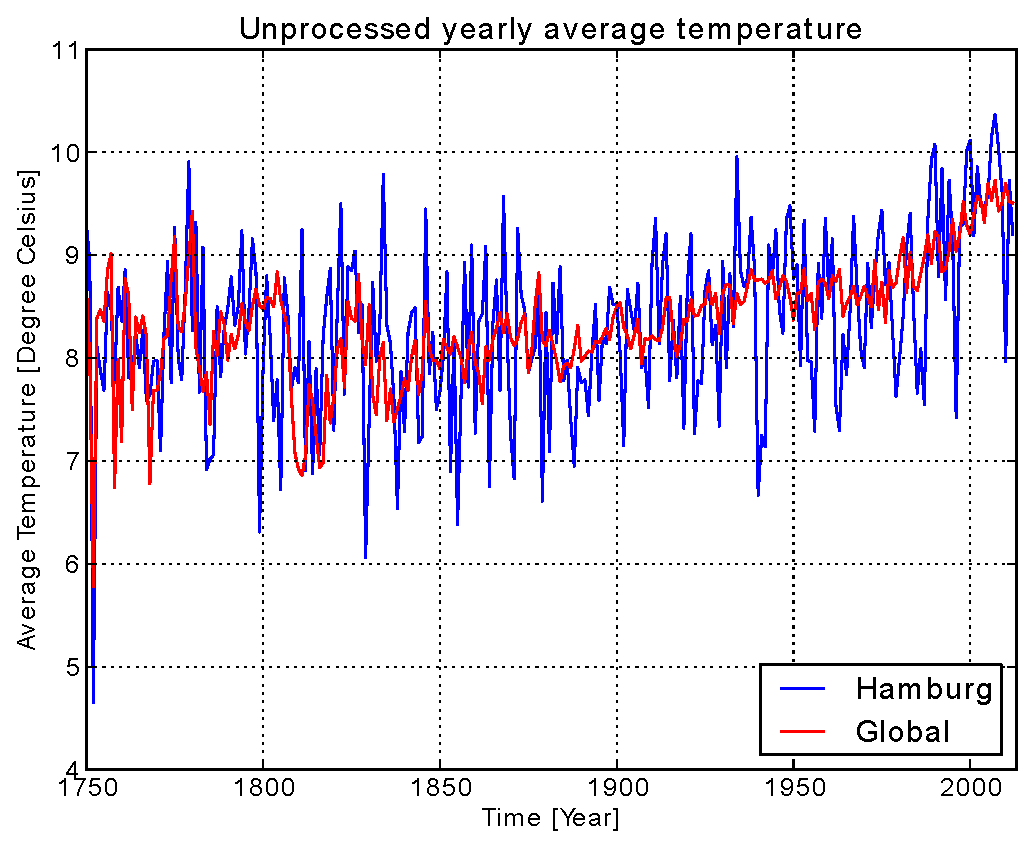
\includegraphics[width=0.75\textwidth]{WeatherTrendsNoisy.eps}
\caption{\label{fig:noisy}Raw (unprocessed) yearly average temperature data of the earth (red) and Hamburg, Germany (blue)}
\end{figure}
More information about the weather trends can be derived by filtering this data. Applying a moving average filter, the raw temperature data can be smoothed. The low-pass filter cuts high-frequency components of the yearly average temperature values to clarify and illustrate the climate's actual development. Figure \ref{fig:filtered} shows the effect of 7-year centered moving average.\\
The variances in global and local temperature values are reduced since outliers have less influence on the results. In the time period from 1750 till the beginning of the $19^{th}$ century, the average temperatures show relatively wide fluctuations resulting in a stabilization and an increasing of the local and global temperatures since 1850. Reasons may be related to the beginning of the industrial revolution and the associated use of fossil fuels as well as the increase of the emission of greenhouse gases. Actually, the temperature rise has increased exponentially for the recent 60 years. Thereby, Hamburg's weather trend follows the global weather trend. Both developments proceed in a similar size and increase.
\begin{figure}
\centering
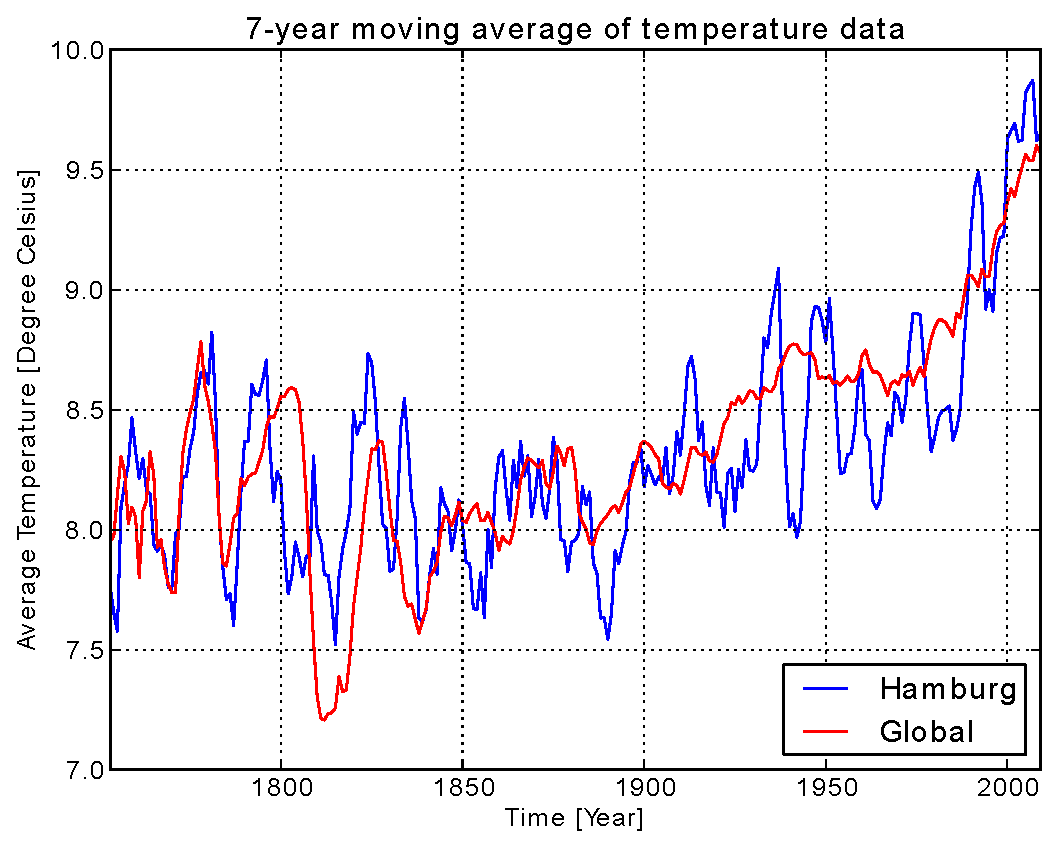
\includegraphics[width=0.75\textwidth]{WeatherTrendsFiltered.eps}
\caption{\label{fig:filtered}Filtered yearly average temperature data of the earth (red) and Hamburg, Germany (blue) using an moving average approach with a window size of $N=7$ years}
\end{figure}
To find the actual increase of the temperatures since 1750, linear regression models are performed. The linear regression models of global $T_{global}(t)$ and local $T_{local}(t)$ temperature data are shown in Figure \ref{fig:LinReg} and the time-dependent mathematical models can be described by applying a least-square algorithm as:
\begin{align}
T_{global}(t)&= 0.00438\cdot t + 0.096 \label{eq:LinRegGlobal}\\
T_{local}(t) &= 0.00372\cdot t + 1.310 \label{eq:LinRegLocal}
\end{align}
The global temperature increase is slightly above the rise of the average temperature in Hamburg. However, an examination of the time period after 1950 using linear regression shows a more drastic increase of the temperature in Hamburg as depicted in Figure \ref{fig:LinReg1950}. The local increase ($0.0261\cdot t$) is much higher than the global temperature rise ($0.0172\cdot t$) and both are many times over the calculated increase in equation \ref{eq:LinRegGlobal} and \ref{eq:LinRegLocal} concerning the recent 260 years.

\begin{figure}
\centering
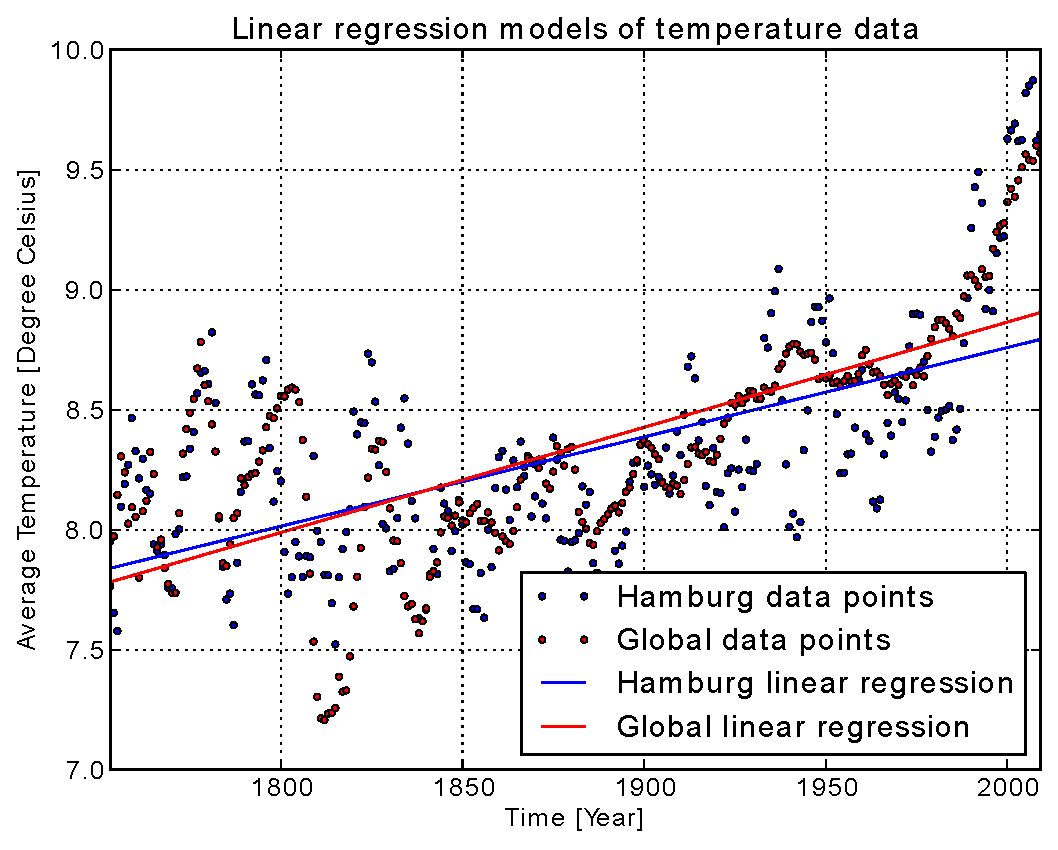
\includegraphics[width=0.75\textwidth]{WeatherTrendsLinReg.eps}
\caption{\label{fig:LinReg}A linear regression model of the yearly average temperature data of the earth (red) and Hamburg, Germany (blue)}
\end{figure}

\begin{figure}
\centering
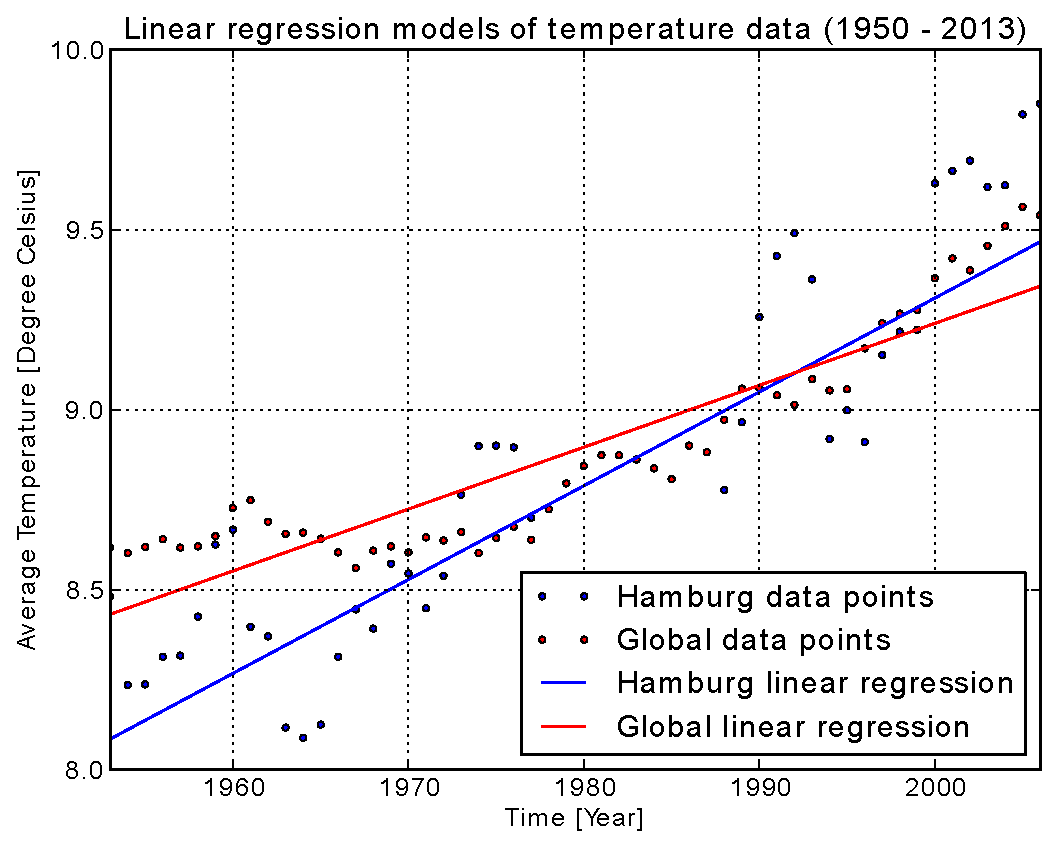
\includegraphics[width=0.75\textwidth]{WeatherTrendsLinReg1950.eps}
\caption{\label{fig:LinReg1950}A linear regression model of the yearly average temperature data of the earth (red) and Hamburg, Germany (blue) since 1950}
\end{figure}

\section{Conclusion}
The examination of weather trend shows an increase of the global yearly average temperature. Especially after the industrial revolution, the temperature on the globe has risen exponentially causing some severe problems regarding environmental and social systems. The comparison between the global climate change and the weather trend in Hamburg, Germany, exhibits great similarities in an overall consideration. The average temperatures of both cases are around the same size. Additionally, the developments of the global and local temperatures appear to behave similarly. Regarding the recent 60 years, Hamburg's yearly average temperature has increased more than the global temperature.  

%
%\begin{thebibliography}{9}
%\bibitem{nano3}
%  K. Grove-Rasmussen og Jesper Nygård,
%  \emph{Kvantefænomener i Nanosystemer}.
%  Niels Bohr Institute \& Nano-Science Center, Københavns Universitet
%
%\end{thebibliography}
\end{document}
